%template author%%%%%%%%%%%%%%%%%%%%%%%%%%%%%%%%%%%%%%%%
% Jacobs Landscape Poster
% LaTeX Template
% Version 1.1 (14/06/14)
%
% Created by:
% Computational Physics and Biophysics Group, Jacobs University
% https://teamwork.jacobs-university.de:8443/confluence/display/CoPandBiG/LaTeX+Poster
% 
% Further modified by:
% Nathaniel Johnston (nathaniel@njohnston.ca)
%
% This template has been downloaded from:
% http://www.LaTeXTemplates.com
%
% License:
% CC BY-NC-SA 3.0 (http://creativecommons.org/licenses/by-nc-sa/3.0/)
%
%%%%%%%%%%%%%%%%%%%%%%%%%%%%%%%%%%%%%%%%%

%----------------------------------------------------------------------------------------
%	PACKAGES AND OTHER DOCUMENT CONFIGURATIONS
%----------------------------------------------------------------------------------------


\documentclass[final]{beamer}

\usepackage[magyar]{babel}
\usepackage[utf8]{inputenc}
\usepackage[style=alphabetic]{biblatex}
%\AtNextBibliography{\small}
%\renewcommand*{\bibfont}{\small}
\renewcommand*{\bibfont}{\tiny}

\bibliography{refs}

\usepackage[scale=1.3]{beamerposter} % Use the beamerposter package for laying out the poster

\usetheme{confposter} % Use the confposter theme supplied with this template

\setbeamercolor{block title}{fg=ngreen,bg=white} % Colors of the block titles
\setbeamercolor{block body}{fg=black,bg=white} % Colors of the body of blocks
\setbeamercolor{block alerted title}{fg=white,bg=dblue!70} % Colors of the highlighted block titles
\setbeamercolor{block alerted body}{fg=black,bg=dblue!10} % Colors of the body of highlighted blocks
% Many more colors are available for use in beamerthemeconfposter.sty

%-----------------------------------------------------------
% Define the column widths and overall poster size
% To set effective sepwid, onecolwid and twocolwid values, first choose how many columns you want and how much separation you want between columns
% In this template, the separation width chosen is 0.024 of the paper width and a 4-column layout
% onecolwid should therefore be (1-(# of columns+1)*sepwid)/# of columns e.g. (1-(4+1)*0.024)/4 = 0.22
% Set twocolwid to be (2*onecolwid)+sepwid = 0.464
% Set threecolwid to be (3*onecolwid)+2*sepwid = 0.708

\newlength{\sepwid}
\newlength{\onecolwid}
\newlength{\twocolwid}
\newlength{\threecolwid}
\setlength{\paperwidth}{48in} % A0 width: 46.8in
\setlength{\paperheight}{36in} % A0 height: 33.1in
\setlength{\sepwid}{0.024\paperwidth} % Separation width (white space) between columns
\setlength{\onecolwid}{0.22\paperwidth} % Width of one column
\setlength{\twocolwid}{0.464\paperwidth} % Width of two columns
\setlength{\threecolwid}{0.708\paperwidth} % Width of three columns
\setlength{\topmargin}{-0.3in} % Reduce the top margin size
%-----------------------------------------------------------

\usepackage{graphicx}  % Required for including images

\usepackage{booktabs} % Top and bottom rules for tables

%https://tex.stackexchange.com/questions/33969/changing-font-size-of-selected-slides-in-beamer
\newcommand\Fontvi{\fontsize{22}{7.2}\selectfont}


%title----------------------------------------------------------------------------------------
%	TITLE SECTION 
%----------------------------------------------------------------------------------------

\title{A comparison of two interaction based random graph models} % Poster title

\author{Cs.Noszály, N.Uzonyi} % Author(s)

\institute{Faculty of Informatics, University of Debrecen} % Institution(s)

%----------------------------------------------------------------------------------------

\begin{document}

\addtobeamertemplate{block end}{}{\vspace*{2ex}} % White space under blocks
\addtobeamertemplate{block alerted end}{}{\vspace*{2ex}} % White space under highlighted (alert) blocks

\setlength{\belowcaptionskip}{2ex} % White space under figures
\setlength\belowdisplayshortskip{2ex} % White space under equations

\begin{frame}[t] % The whole poster is enclosed in one beamer frame

\begin{columns}[t] % The whole poster consists of two major columns, each of which is split into two columns - the [t] option aligns each column's content to the top

\begin{column}{\sepwid}\end{column} % Empty spacer column


%%%%%%% 1 col
\begin{column}{\twocolwid} % Begin a column which is two columns wide (column 1)

%%%%%%% split of 1 col
\begin{columns}[t,totalwidth=\twocolwid] % Split up the two columns wide column

%%%%%%% 1.1 col
\begin{column}{\onecolwid}\vspace{-.6in} % The first column within column 1 (column 1.1)

% the model description
\begin{block}{The N-clique model}\small

  Backhausz and Móri in \cite{BaMo} introduced a new class of random graphs based on interactions of three vertices. They proved almost sure results exhibiting the scale free property. The model and the results were further generalized by Fazekas and Porvázsnyik in \cite{FaPo}. Here is a short recipe of the generation: Start with an $N$-clique, with weigths one all of its subcliques. At each step $N$ vertices interact. W.p. (i.e. with probabilty) $p$ add a new vertex $v$ to the graph and select an $N-1$ element set $K$ from the old vertices: w.p. $r$ from the $N-1$ cliques proportional to their weights or w.p. $1-r$ from the existing vertices uniformly, then set $K=K\cup{v}$. W.p. $1-p$ select an $N$ element set $K$ from the old vertices: w.p. $q$ select from the $N$ cliques proportional to their weights or w.p. $1-q$ from the existing vertices uniformly. In ether cases add the $N$-clique generated by $K$ to the graph and increase all of its subcliques weights by one.

\end{block}


% scale-freeness
\begin{block}{Scale-free property}\centering
  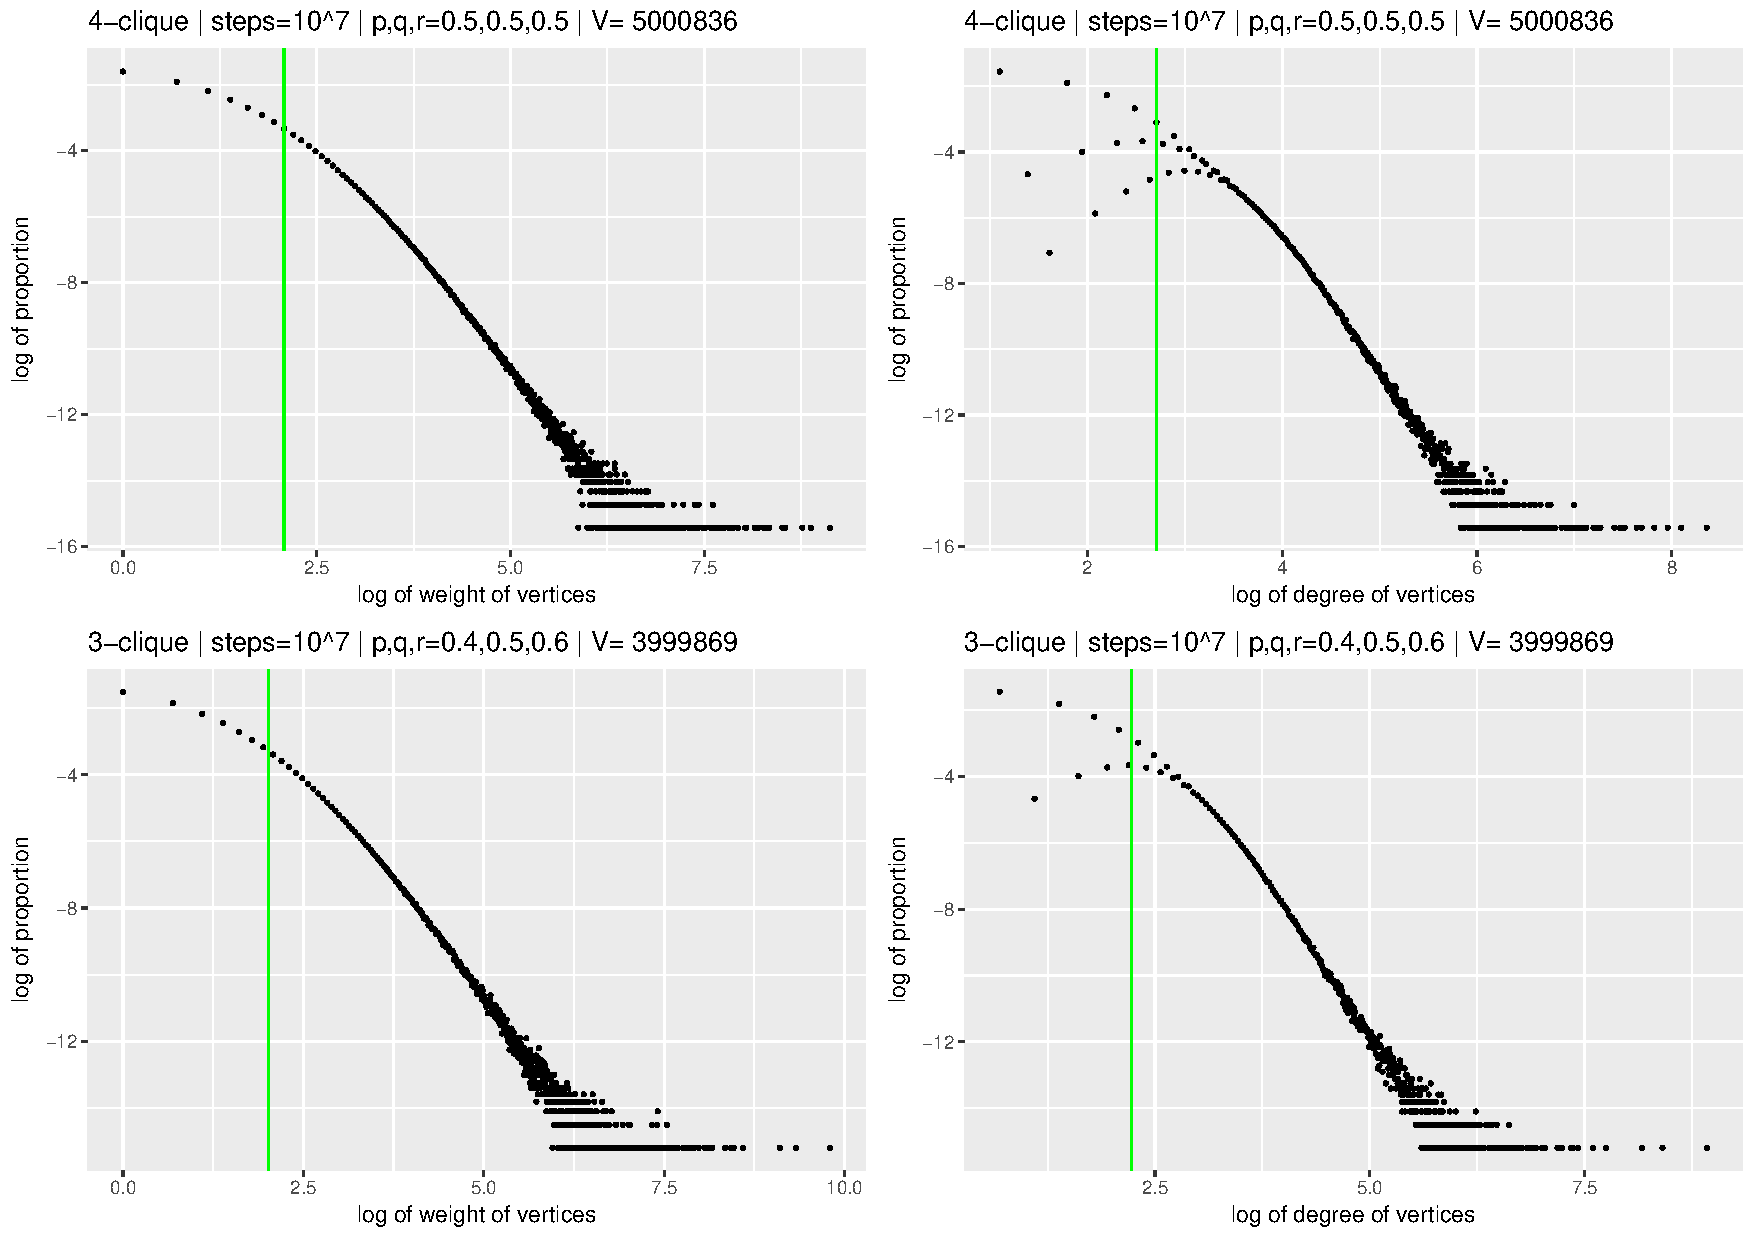
\includegraphics[width=0.8\linewidth]{./fig/klikkdist4.pdf}
\end{block}


% small-world
\begin{block}{Small-world property}\small
Finding the exact diameter of large graphs is a computationally intensive task. We implemented the method proposed in \cite{CreMa}. The algorithm iteratively refines the lower and upper bound for the given graph using breadth first searches. We generated ca. 1000 instances of the $N$-clique models for various parameters, and determined the additive $2$-approximations of the diameter. In the figures the red and blue marks are the upper and lower bounds for $\frac{diam(G(V,E))}{\log(|V|)}$. From practical point of view one can conclude that the diameter is in $O(\log(|V|))$.
\end{block}



\end{column} % End of column 1.1


%%%%%%% 1.2 col
\begin{column}{\onecolwid}\vspace{-.6in} % The second column within column 1 (column 1.2)


% clustering coefficient
\begin{center}
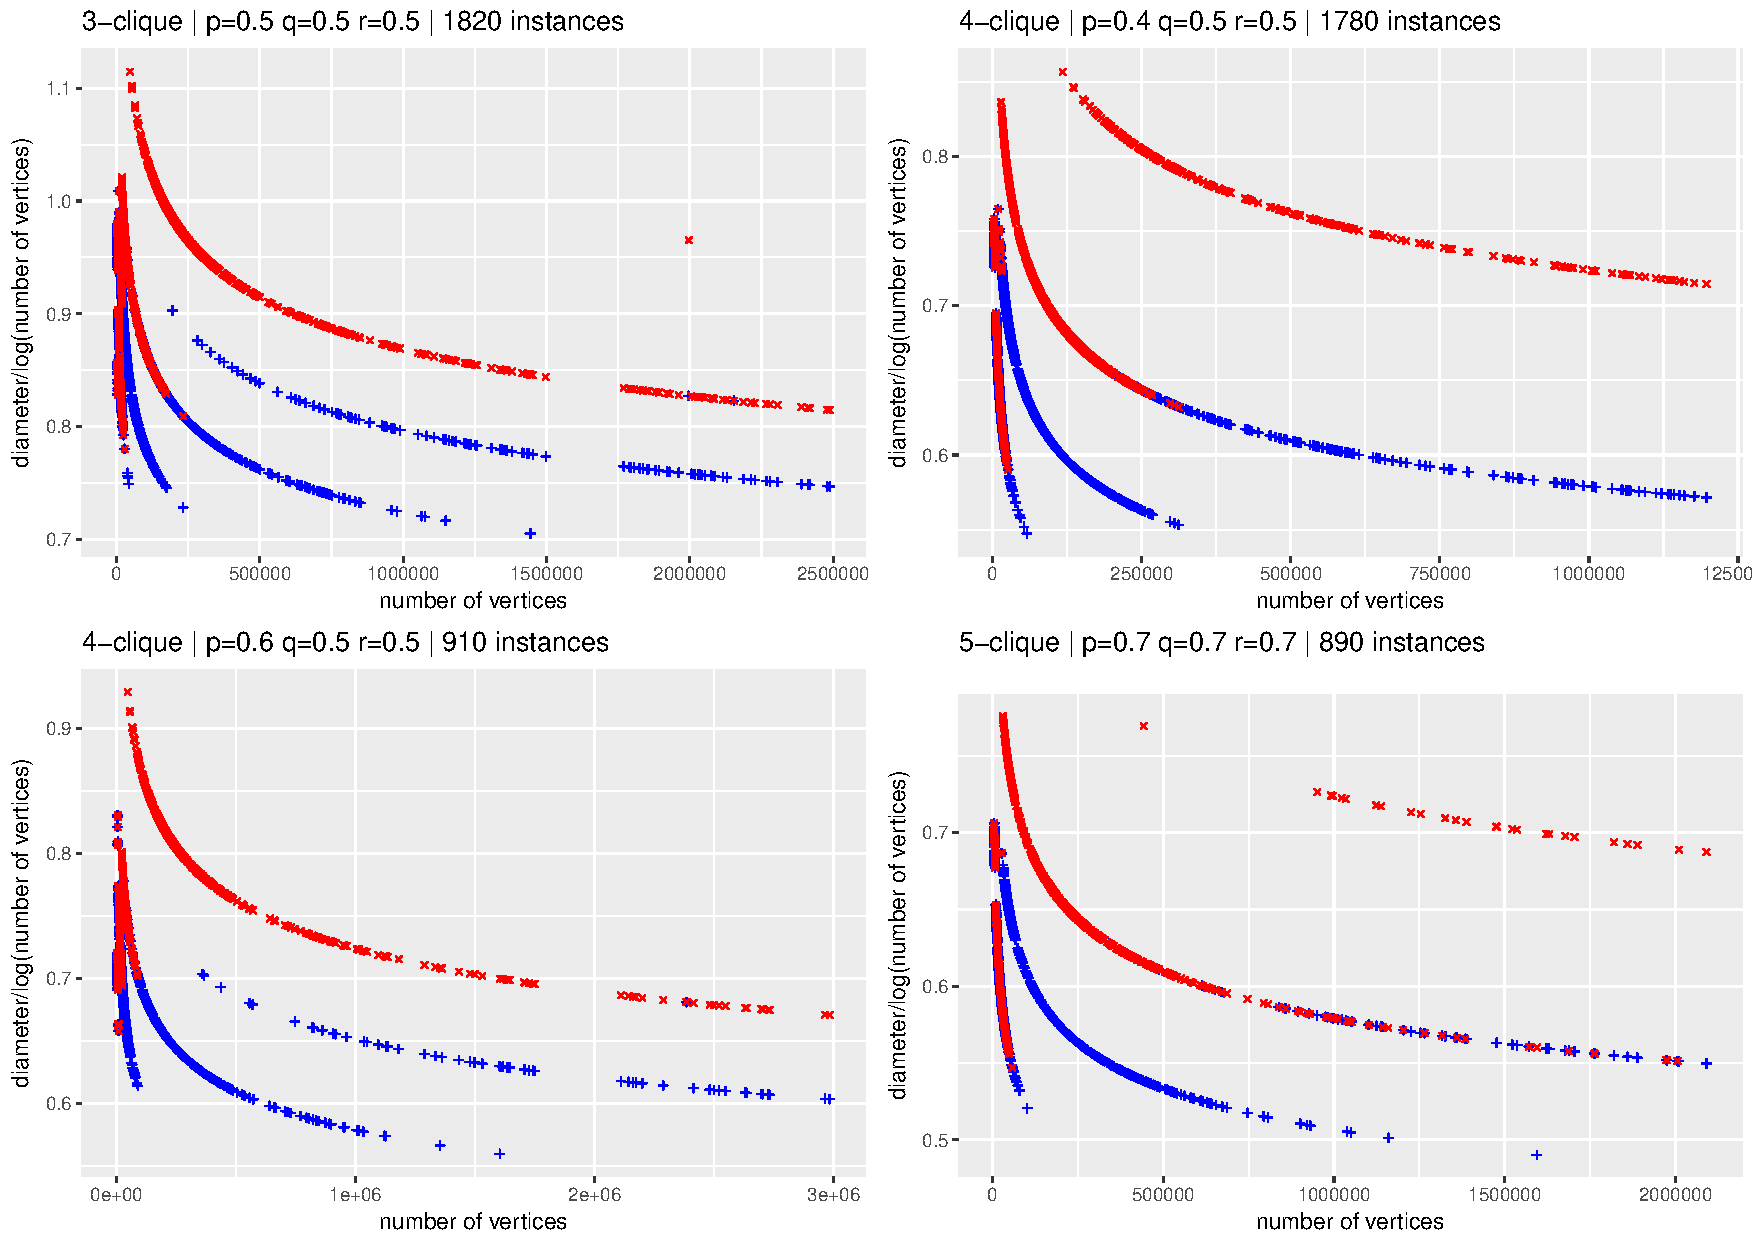
\includegraphics[width=0.8\linewidth]{./fig/klikkdiam4.pdf}
\end{center}

  
\begin{block}{Clustering coefficient}
\small
  The local clustering coefficient of a node $v$, is a proportion of connected vertex pairs among all possible pairs from the neighbourhood of $v$. Its exact computations are basically triangle counting methods see \cite{Lat}. We implemented an $O(|V|maxdeg^{2})$ algorithm.
  
  \vskip 1cm
  \centering
  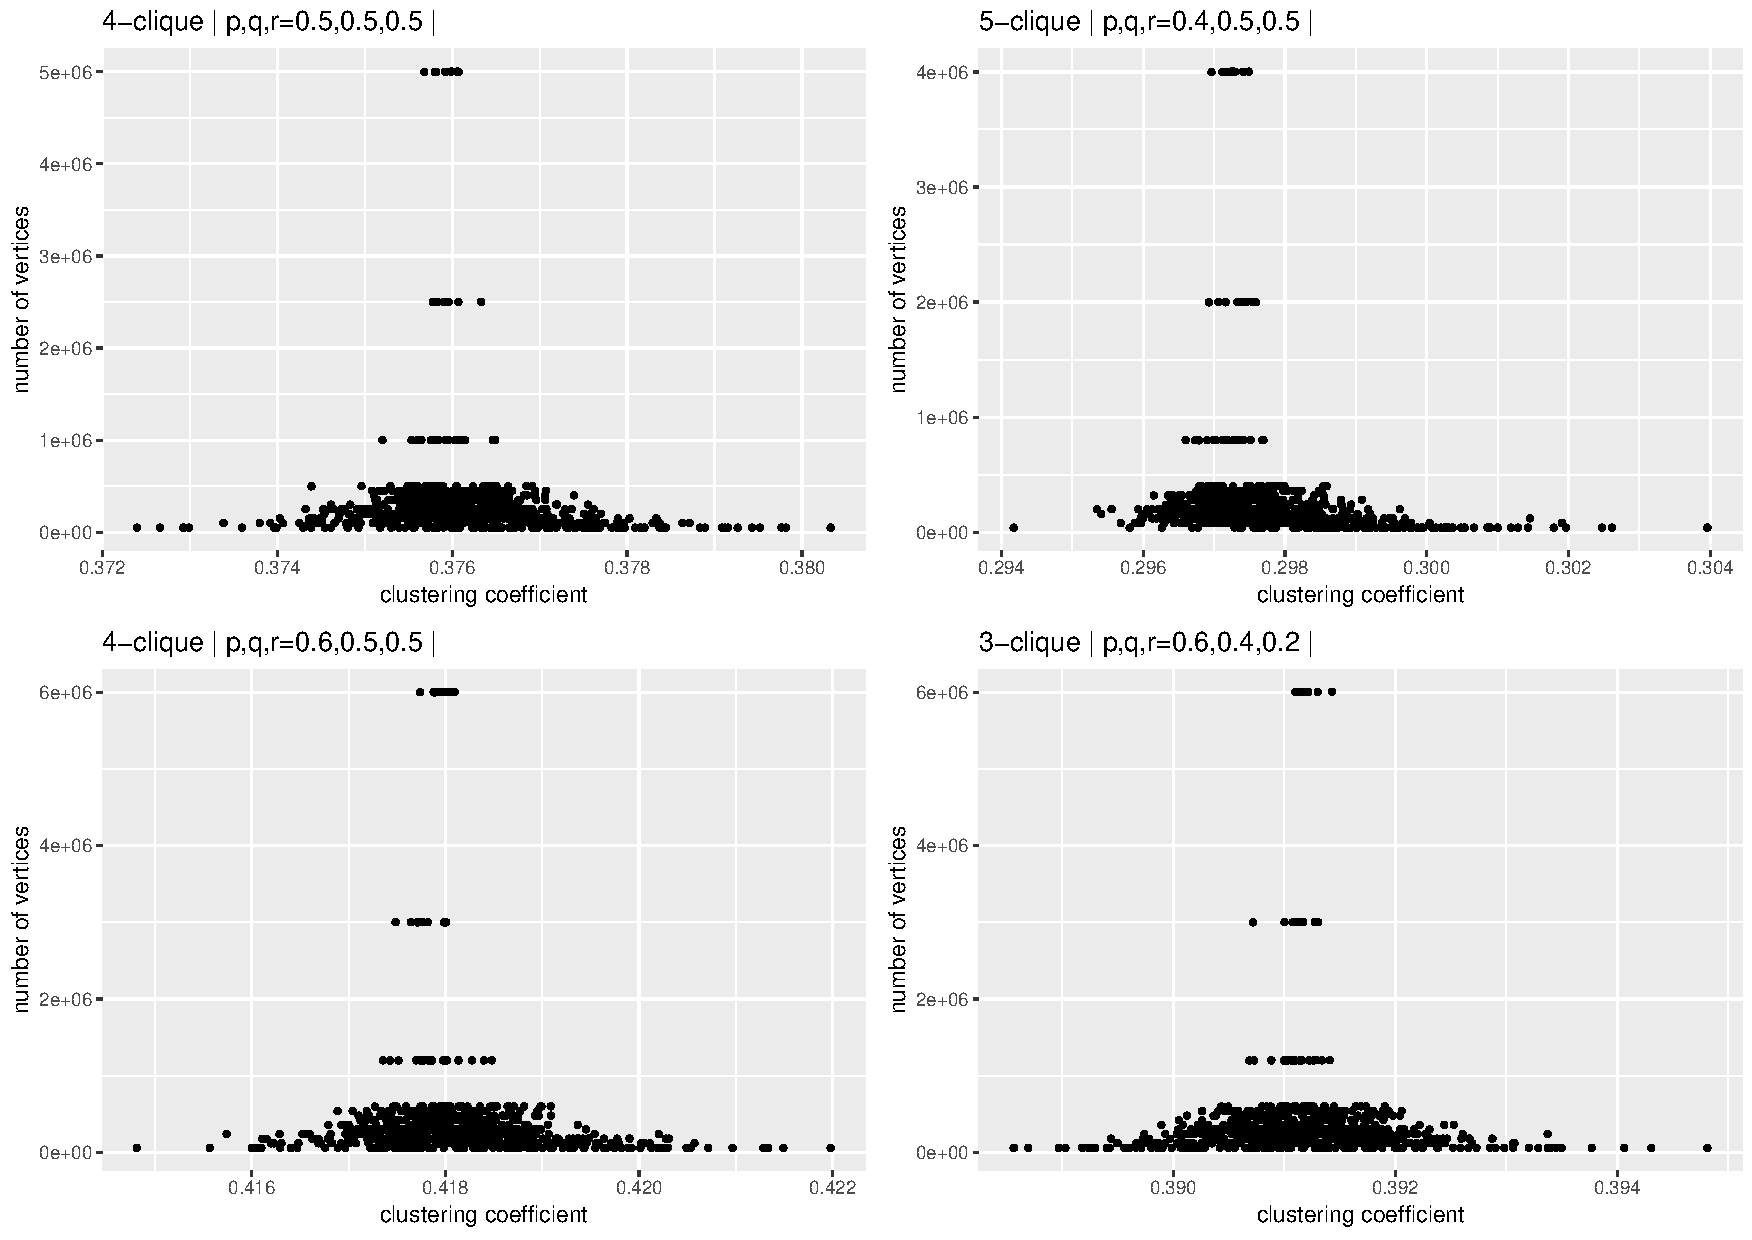
\includegraphics[width=0.8\linewidth]{./fig/klikkclust4.pdf}
\end{block}


\end{column}

\end{columns} % End of the split of column 1

%% \begin{column}{\twocolwid}
%% \begin{block}{valami}

%% \end{block}
%% \end{column}

\end{column}%bal oszlop

\begin{column}{\sepwid}\end{column} % Empty spacer column

%%%%%%% 2 col
\begin{column}{\twocolwid} % Begin a column which is two columns wide (column 2)

%%%%%%% split of 2
\begin{columns}[t,totalwidth=\twocolwid] % Split up the two columns wide column

%%%%%%% 2.1 col
\begin{column}{\onecolwid}\vspace{-.6in} % The first column within column 2 (column 2.1)
  
% the model description
\begin{block}{The N-star model}\small
  
  It is a centralized variant of the $N$-clique model: at each step a (possibly new) vertex and $N-1$ old vertices interact forming an $N$-star, i.e an $N$-tree with a central vertex and $N-1$ leaves.
  The process of the evolution is as follows: Start with an $N$-star, with weigths one all of its substars. At each step $N$ vertices interact. W.p. $p$ add a new vertex $v$ to the graph and select an $N-1$ element set $K$ from the old vertices: w.p. $r$ from the $N-1$ stars proportional to their weights or w.p. $1-r$ from the existing vertices uniformly, then set $K=K\cup{v}$. W.p. $1-p$ select $N$ element set $K$ from the old vertices: w.p. $q$ select from the $N$ stars proportional to their weights or w.p. $1-q$ from the existing vertices uniformly.  Note that if no central node in $K$ ($(p,1-r)$ and $(1-p,1-q)$ branches) select it uniformly from the {\small\it old} vertices of $K$. At last add the $N$-star generated by $K$ to the graph and increase all of its substars weights by one.
\end{block}


% scale-freeness
\begin{block}{Scale-free property}
\begin{figure}
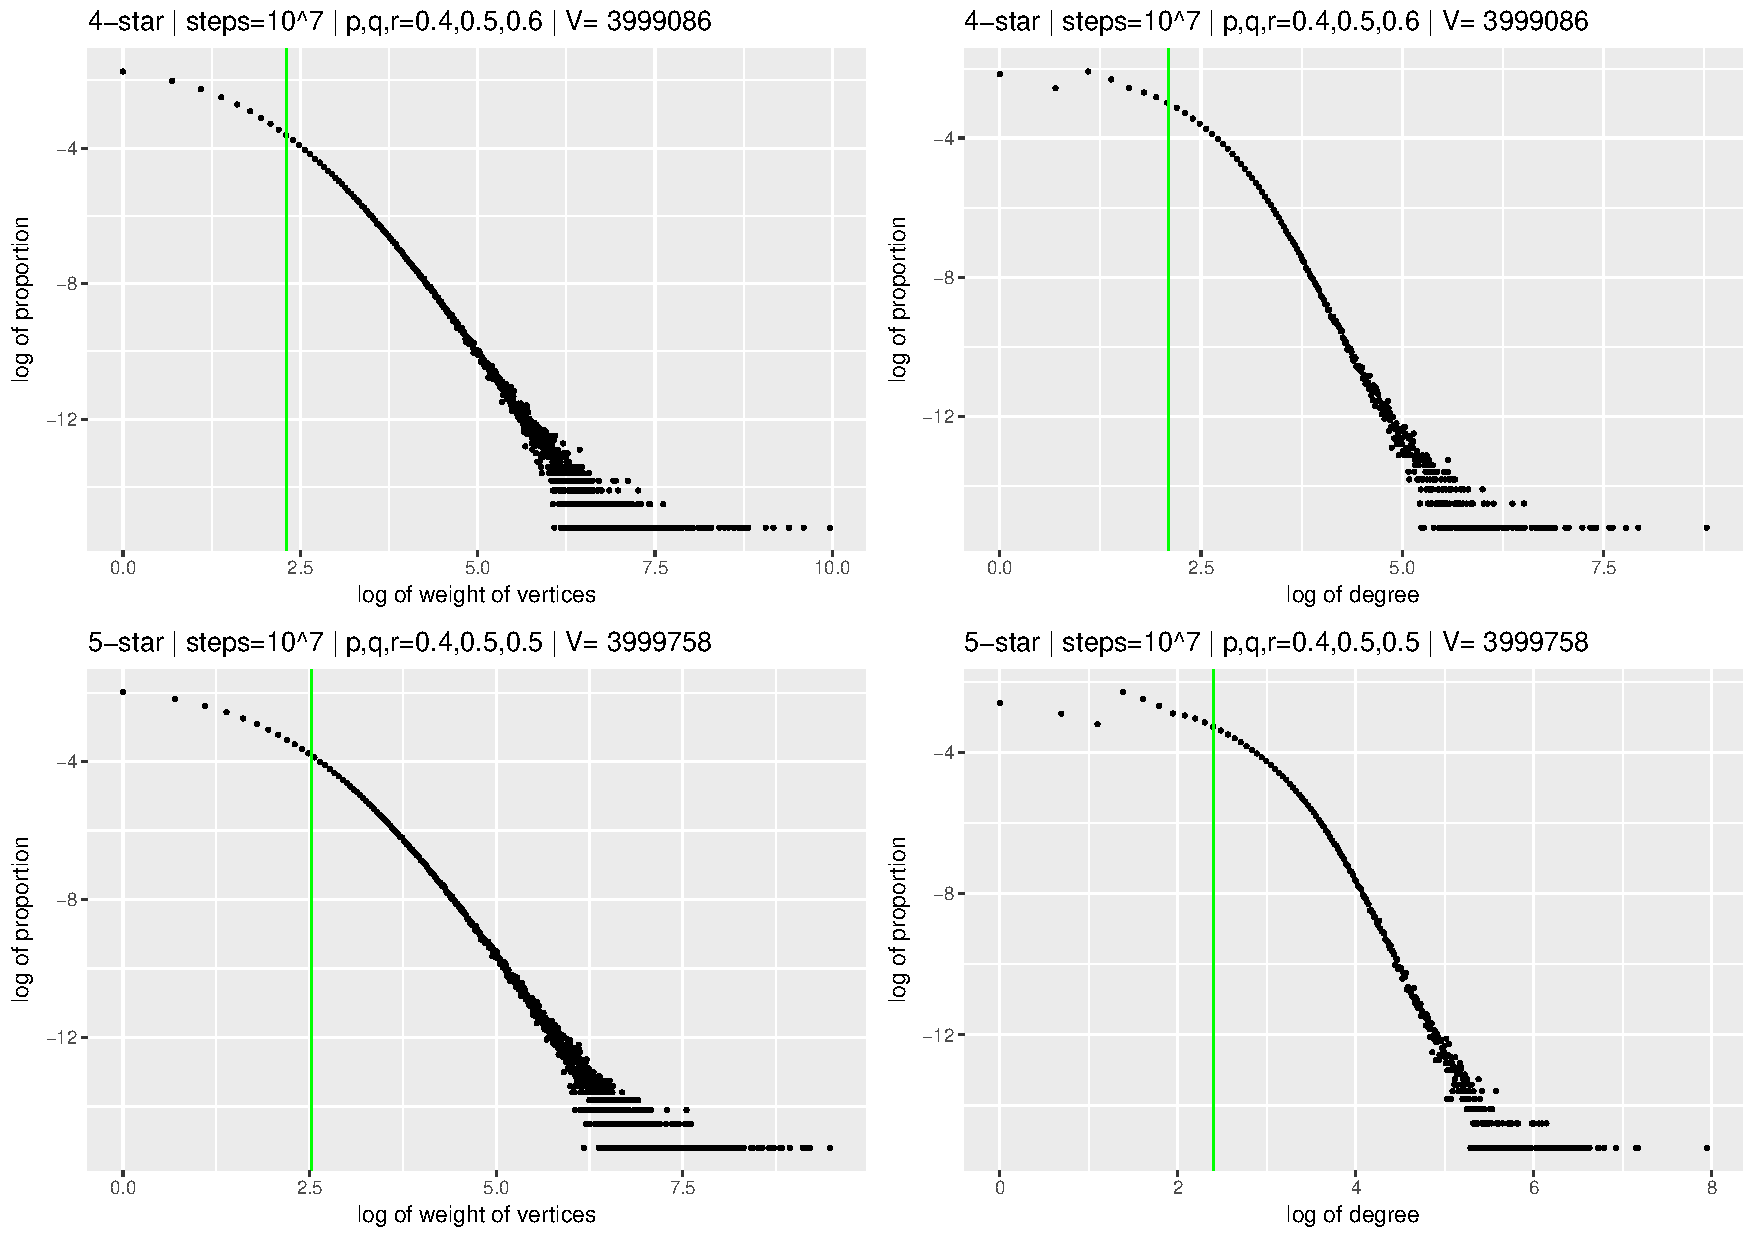
\includegraphics[width=0.8\linewidth]{./fig/csilldist4.pdf}
\end{figure}
\end{block}


% small-world
% small-world
\begin{block}{Small-world property}
  \centering
  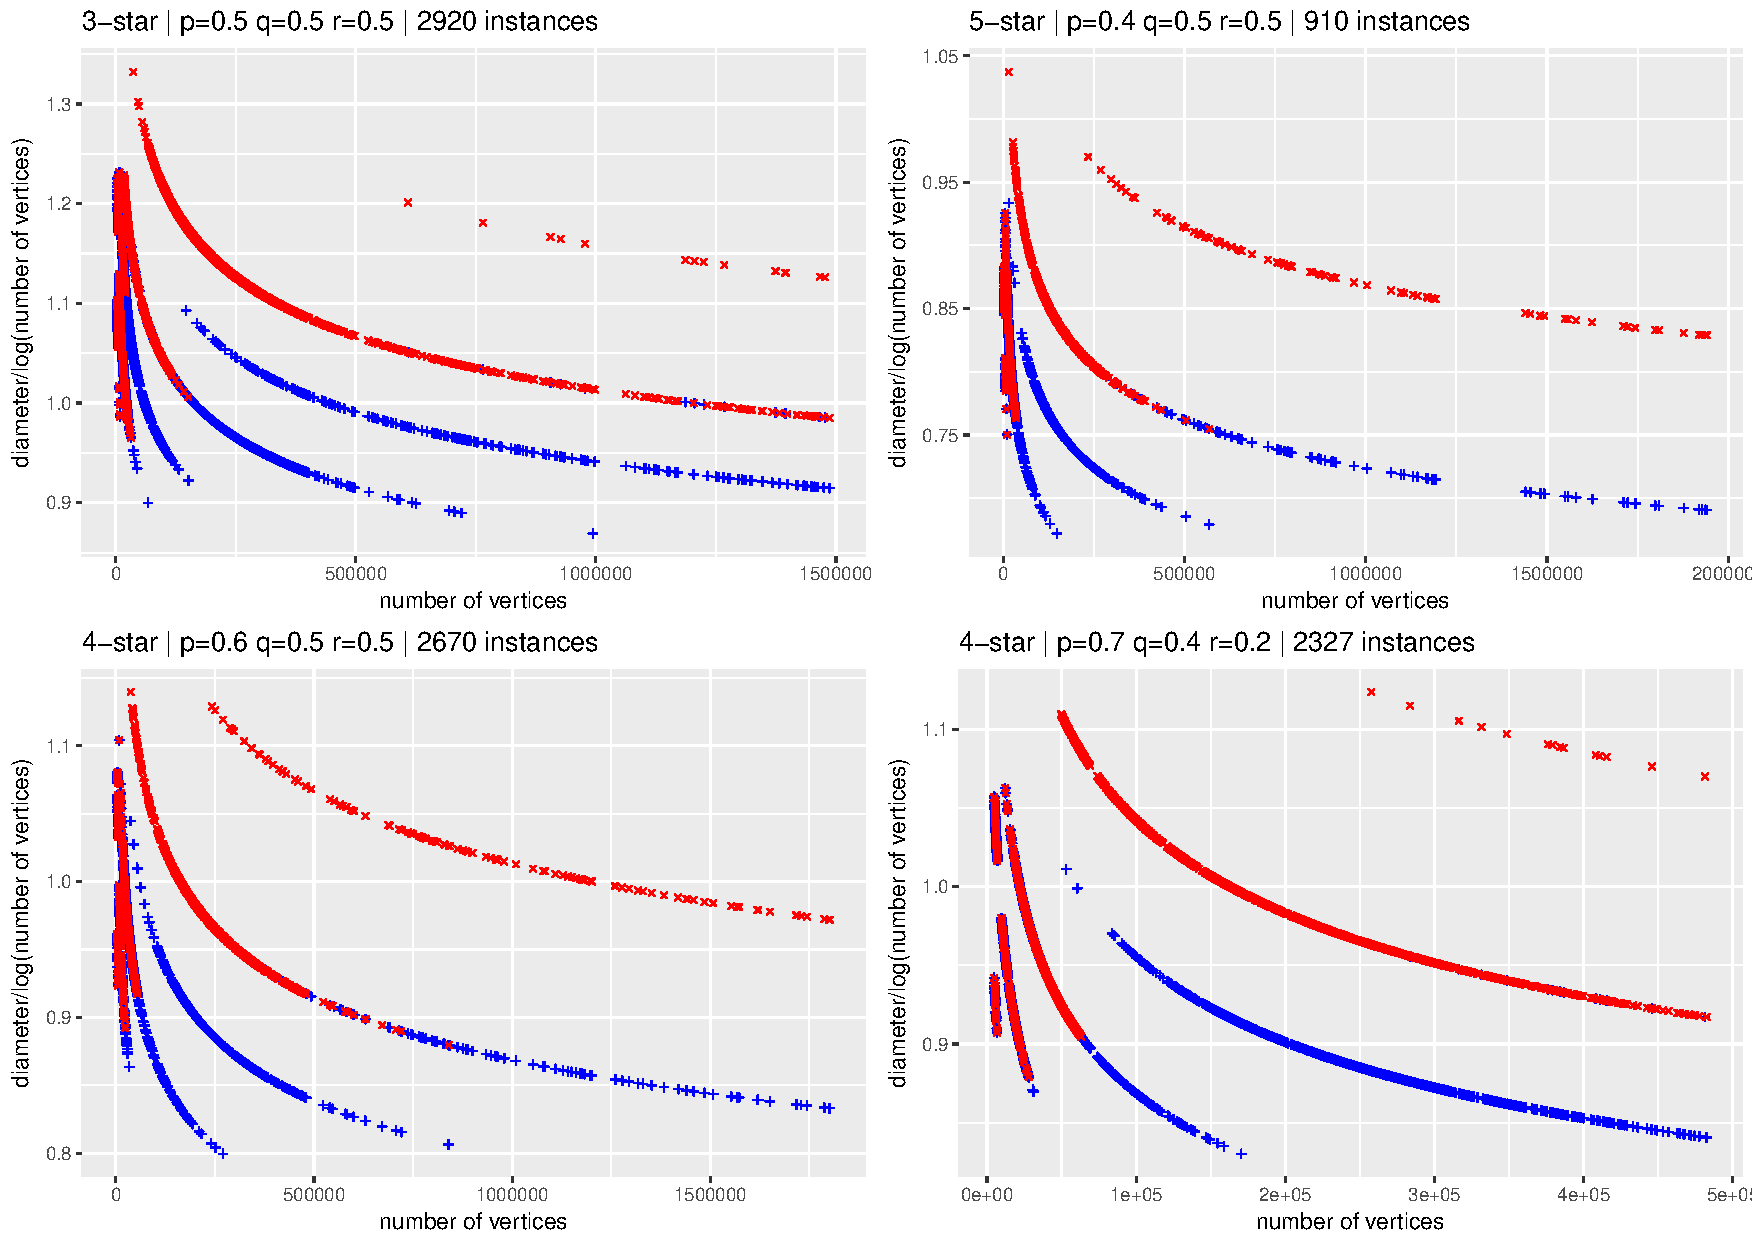
\includegraphics[width=0.8\linewidth]{./fig/csilldiam4.pdf}
\end{block}


  
\end{column} % End of column 2.1


%%%%%%% 2.2 col
\begin{column}{\onecolwid}\vspace{-.6in} % The second column within column 2 (column 2.2)
% clustering coefficient
% clustering
\begin{block}{Clustering coefficient}
\begin{figure}
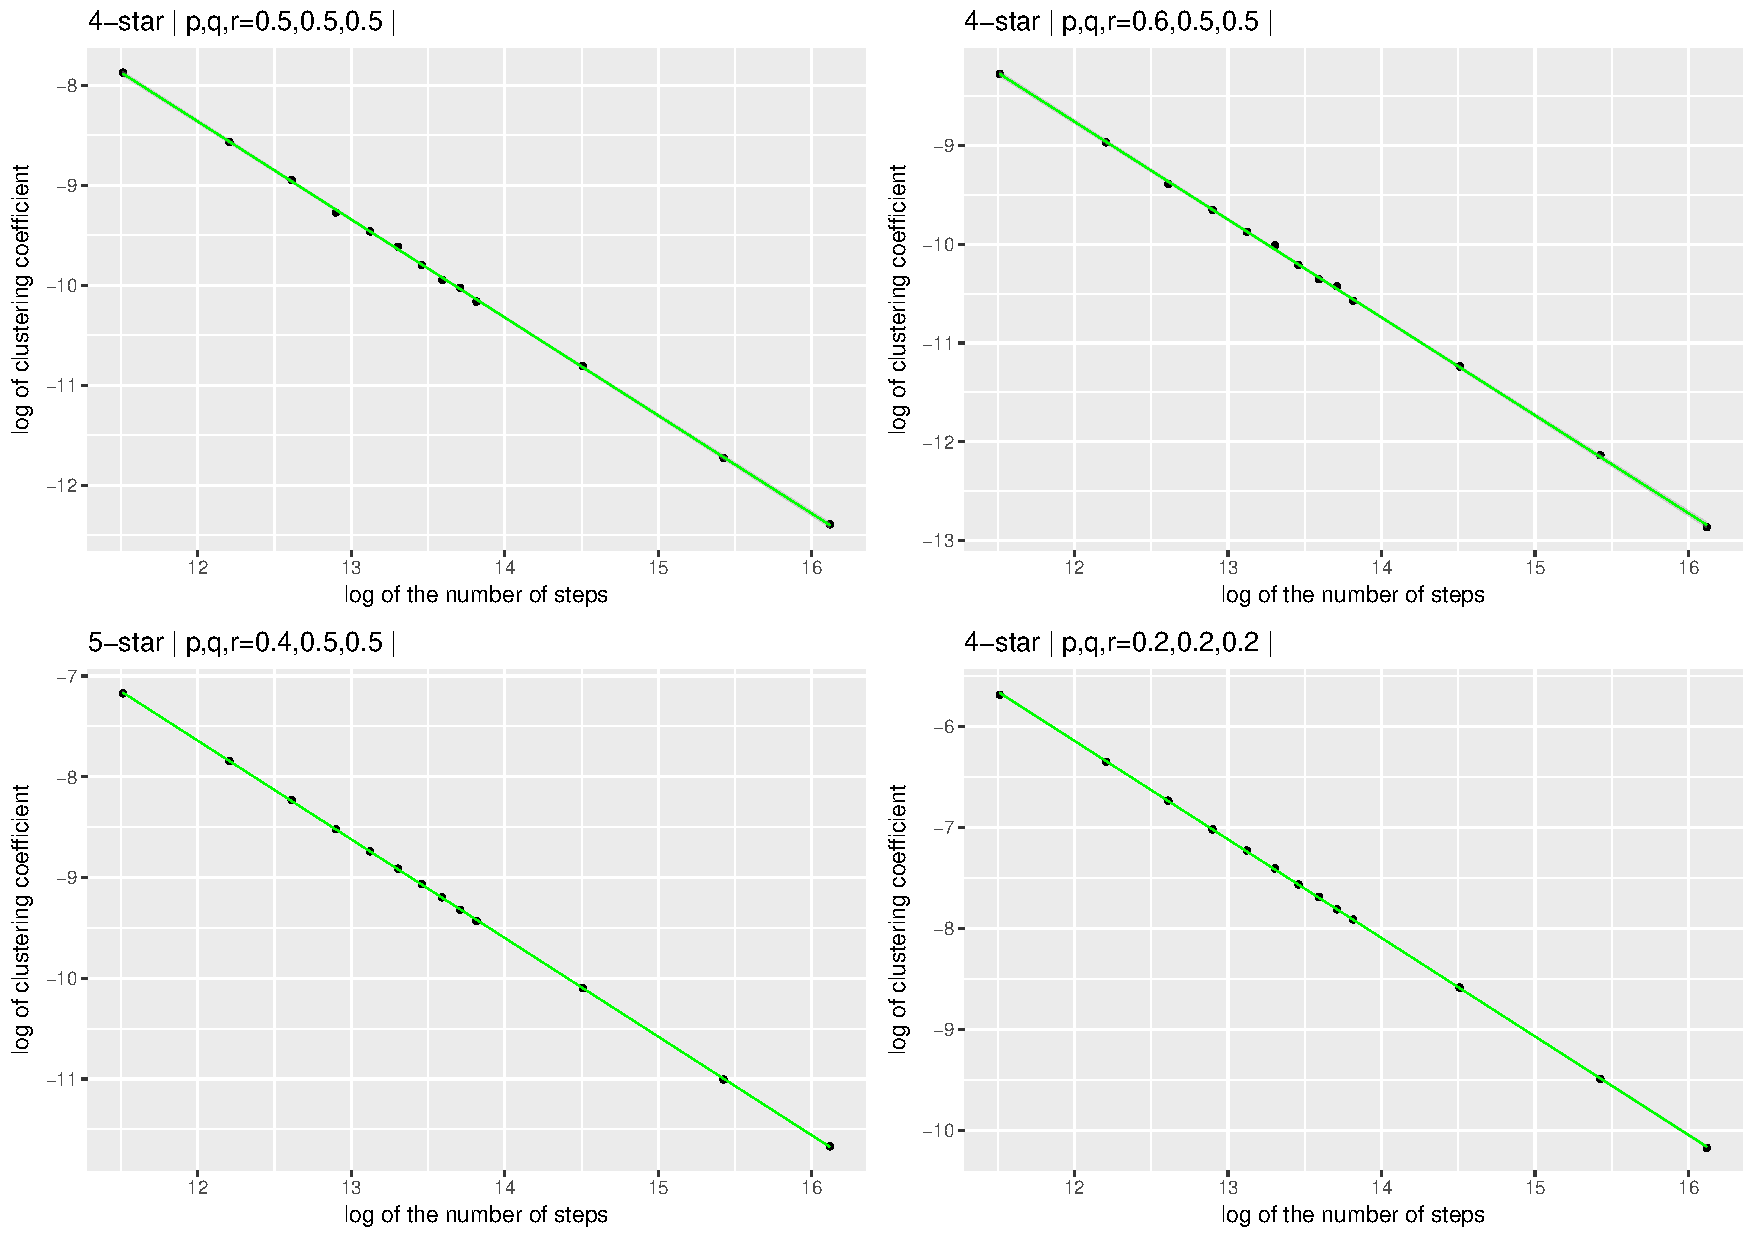
\includegraphics[width=0.8\linewidth]{./fig/csillclustlog4.pdf}
%\caption{Figure caption}
\end{figure}
\end{block}


  
\begin{block}{References}
\printbibliography
\end{block}

%----------------------------------------------------------------------------------------

\end{column} % End of column 2.2

\end{columns} % End of the split of column 2 - any content after this will now take up 2 columns width


\end{column} % end of col 2

\end{columns} % End of all the columns in the poster

\end{frame} % End of the enclosing frame

\end{document}
